\documentclass[10pt]{article}

% Pacotes extras necessários
\usepackage{amsmath}
\usepackage[lmargin=0.5in, rmargin=0.5in, tmargin=0.5in, bmargin=0.5in, includehead, includefoot]{geometry}
\usepackage{amsfonts}
\usepackage[utf8]{inputenc}
\usepackage[portuguese]{babel}
\usepackage{graphicx}
\usepackage{fancyhdr}
\usepackage{setspace}
\usepackage{listings}
\usepackage{url}
\usepackage{enumitem}
\usepackage{appendix}
\usepackage{subcaption}
\usepackage[dvipsnames]{xcolor}
\usepackage{tikz}
\usepackage{makecell}
\usetikzlibrary{positioning}

% Define estilo para listagens de código
\lstdefinestyle{mystyle}{
    language=Matlab,
    inputencoding=latin1,
    extendedchars=true,
    backgroundcolor=\color{white},
    basicstyle=\ttfamily\footnotesize,
    numbers=left,
    numberstyle=\tiny\color{gray},
    numbersep=5pt,
    tabsize=2,
    breaklines=true,
    keywordstyle=\color{blue},
    commentstyle=\color{green!60!black},
    stringstyle=\color{orange},
    frame=single,
    keepspaces=true,
    showspaces=false,
    showstringspaces=false,
    showtabs=false,
}
\lstset{style=mystyle}

\graphicspath{{./images/}}

\setlength{\parindent}{0pt}
\setstretch{1.5}

\DeclareMathOperator{\sen}{sen}
\DeclareMathOperator{\sinc}{sinc}
\newcommand{\Lap}[1]{\mathcal{L}\left\{#1\right\}}
\newcommand{\bm}[1]{\boldsymbol{#1}}

% Cabeçalho e rodapé em todas as páginas
\pagestyle{fancy}
\fancyhf{}
\fancyhead[L]{Relatório das simulações}
\fancyfoot[C]{\thepage}

% Dados do Grupo
\title{
    Trabalho Nº 03 - Solução do controle 2DOF \\
    \large COE603 - Controle Adaptativo
}
\author{
    Caio Cesar Leal Verissimo - 119046624 \\
    Leonardo Soares da Costa Tanaka - 121067652 \\
    Lincoln Rodrigues Proença - 121076407 \\
    Engenharia de Controle e Automação - UFRJ \\
    Rio de Janeiro, Rio de Janeiro, Brasil \\
    Julho de 2025
}
\date{}

\begin{document}

\maketitle

% Geração automática do sumário
\tableofcontents
\newpage

\section{Descrição do Algoritmo}

Nesta seção, descrevemos o algoritmo de controle baseado na estrutura 2DOF (Two Degrees of Freedom) utilizando MRAC (Model Reference Adaptive Control).
Conforme ilustrado nas figuras apresentadas ao longo da seção.

\begin{figure}[h!]
    \centering
    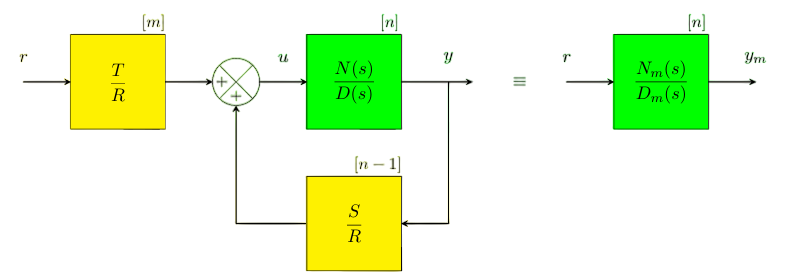
\includegraphics[width=0.65\textwidth]{img/controle2dof.png}
    \caption{Estrutura do controlador 2DOF.}
    \label{fig:2dof_structure}
\end{figure}

\subsection{Lei de Controle Linear}

A lei de controle na estrutura 2DOF é dada por:
\[
Ru = Tr + Sy \quad \Rightarrow \quad u = \frac{T}{R}r + \frac{S}{R}y
\]

Para o caso em que o grau relativo $n^* = 1$, pode-se usar a estrutura com \textbf{feedforward}, onde:
\[
\frac{T}{R} = \frac{N_m}{D_m} \quad \Rightarrow \quad R = N
\]

Contudo, como $N(s)$ é desconhecido, não pode aparecer no denominador. A solução é utilizar uma estrutura com filtros, conforme apresentada a seguir.

\begin{figure}[h!]
    \centering
    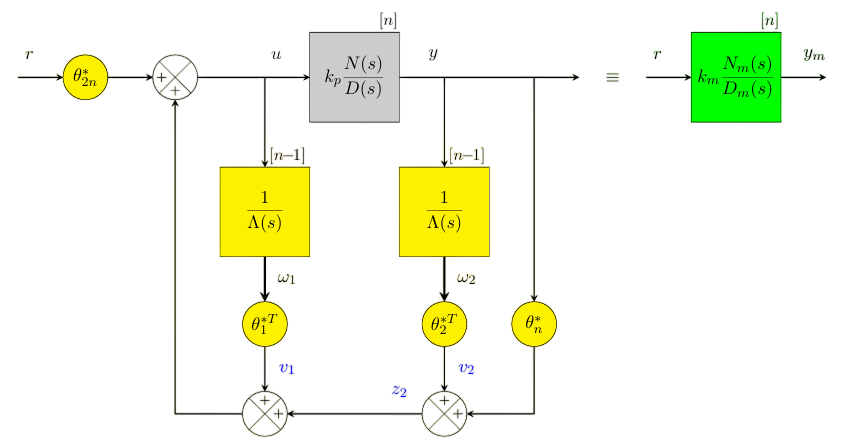
\includegraphics[width=0.65\textwidth]{img/estrutura_mrac.png}
    \caption{Estrutura do MRAC com filtros.}
    \label{fig:mrac_structure}
\end{figure}

\subsection{Filtros}

\begin{itemize}
    \item \textbf{Filtro 1:}
    \[
    \begin{cases}
        \dot{\omega}_1 = A_f \omega_1 + b_f u \\
        v_1 = \theta_1^{*T} \omega_1 
    \end{cases}
    \quad \Rightarrow \quad v_1 = \frac{F}{\Lambda} u \quad  \left[ grau(F)=n-2 \right]
    \]
    \item \textbf{Filtro 2:}
    \[
    \begin{cases}
        \dot{\omega}_2 = A_f \omega_2 + b_f y \\
        z_2 = \theta_2^{*T} \omega_2 + \theta_n^* y
    \end{cases}
    \quad \Rightarrow \quad z_2 = \frac{G}{\Lambda} y \quad  \left[ grau(G)=n-1 \right]
    \]
\end{itemize}

\subsection{Lei de Controle Adaptativa}

A lei de controle pode ser escrita como:
\[
u = \theta^{*T} \omega
\]
com:
\[
\theta^* = \begin{bmatrix}
\theta_1^* & \theta_n^* & \theta_2^* & \theta_{2n}^*
\end{bmatrix}^{T}, \quad \theta^* \in \mathbb{R}^{2n}, \quad 
\omega = \begin{bmatrix}
\omega_1 & y & \omega_2 & r
\end{bmatrix}^{T}, \quad \omega \in \mathbb{R}^{2n}
\]

\subsection{Simplificação da Estrutura}

A estrutura pode ser simplificada a partir da relação:
\[
u = z_1 + \frac{F}{\Lambda} u \quad \Rightarrow \quad (\Lambda - F) u = \Lambda z_1 \quad \Rightarrow \quad u = \frac{\Lambda}{\Lambda - F} z_1
\]

\begin{figure}[h!]
    \centering
    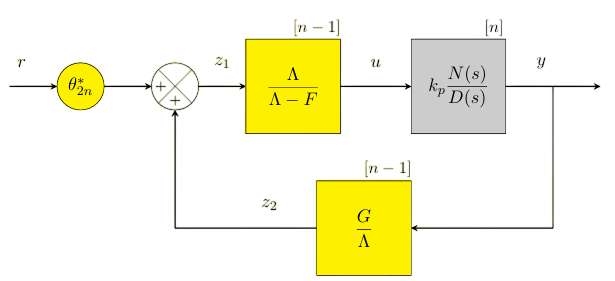
\includegraphics[width=0.65\textwidth]{img/mrac_simplified.png}
    \caption{Reorganização da estrutura MRAC.}
    \label{fig:mrac_simplified}
\end{figure}

\newpage

\subsection{Malha Fechada e Condições de Matching}

\begin{figure}[h!]
    \centering
    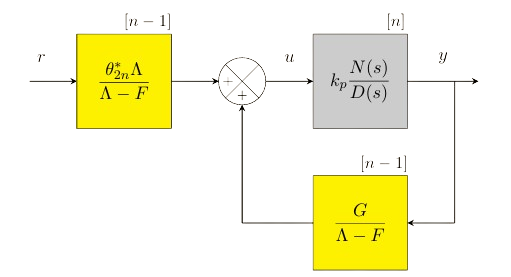
\includegraphics[width=0.65\textwidth]{img/malha_fechada.png}
    \caption{Diagrama da malha fechada com os filtros.}
    \label{fig:closed_loop_mrac}
\end{figure}

A expressão da malha fechada, considerando a estrutura com filtros, é dada por:
\[
y = k_p\frac{N}{D} \left( \frac{\theta_{2n}^* \Lambda}{\Lambda - F} r + \frac{G}{\Lambda - F} y \right)
\]

Multiplicando ambos os lados por $D(\Lambda - F)$, obtemos:
\[
D(\Lambda - F) y = \theta_{2n}^* k_p \Lambda N r + k_p N G y
\]

Reorganizando:
\[
y = \frac{\theta_{2n}^* k_p \Lambda N}{(\Lambda - F)D - k_p N G} r
\]

\textbf{Matching antes dos cancelamentos:}

Deseja-se realizar o \textit{matching} com a função de transferência de referência:
\[
\frac{\theta_{2n}^* k_p \Lambda N}{(\Lambda - F)D - k_p N G} = \frac{k_m N_m}{D_m}
\]

Ou seja:
\[
\theta_{2n}^* k_p \Lambda N D_m = k_m N_m N A_0 \quad \text{(numerador)}
\]
\[
D(\Lambda - F) - k_p N G = D_m A_0 \quad \text{(denominador)}
\]

\textbf{Condições necessárias para o matching:}
\begin{itemize}
    \item $\theta_{2n}^* = \dfrac{k_m}{k_p}$
    \item $\Lambda = N_m A_0$
\end{itemize}

\textbf{Graus dos polinômios envolvidos:}
\[
\begin{cases}
    grau(\Lambda) = n - 1 \\
    grau(N_m) = m
\end{cases} \Rightarrow grau(A_0) = n - m - 1 = n^* - 1
\]

Para cancelar $N$ no denominador da função de transferência, requer-se:
\[
\Lambda - F = N H
\]

\[
\begin{cases}grau(\Lambda) = n - 1 \\
    grau(F) = n - 2 \\
    grau(N) = m
\end{cases} \Rightarrow grau(H) = n - m - 1 = n^* - 1
\]

\textbf{Hipóteses adicionais:}
\begin{itemize}
    \item $P$ é controlável e observável.
    \item $N$ e $D$ são primos entre si.
\end{itemize}

\subsection{Equação Diofantina}

A partir dos cancelamentos necessários, obtemos a equação:
\[
H(s)D(s) - k_p G(s) = D_m(s) A_0(s)
\]

Analisando os graus dos polinômios envolvidos, temos:

\begin{itemize}
    \item $grau(HD) = grau(H) + grau(D) = (n - m - 1) + n = 2n - m - 1$
    \item $grau(G) = n - 1$
    \item $grau(D_m A_0) = grau(D_m) + grau(A_0) = n + (n - m - 1) = 2n - m - 1$
    \item $H(s)$ é um polinômio monônico
\end{itemize}

\textbf{Hipótese importante:} O grau relativo de $P(s)$ é igual ao grau relativo de $M(s)$:
\[
grau(D) - grau(N) = grau(D_m) - grau(N_m) = n^*
\]

\noindent
\textbf{Observação:} O grau relativo é uma propriedade invariante e fundamental para o projeto correto do controlador adaptativo.

\subsection{Resumo do Algoritmo}

\begin{enumerate}
    \item Determinar os graus de $A_0(s)$ e $G(s)$.
    \item Resolver a equação Diofantina: 
    \[
    H(s)D(s) - k_p G(s) = D_m(s)A_0(s)
    \]
    \item Obter $\theta_2^*$ e $\theta_n^*$ a partir de $G(s)$.
    \item Calcular $F(s)$ pela relação: 
    \[
    F(s) = \Lambda(s) - N(s)H(s)
    \]
    \item Obter $\theta_1^*$ a partir de $F(s)$.
    \item Obter $\theta_{2n}^*$ via: 
    \[
    \theta_{2n}^* = \frac{k_m}{k_p}
    \]
\end{enumerate}

\section{Implementação do Algoritmo}

\newpage

\section{Teste da Implementação}

\subsection{Teste (\texorpdfstring{$n^* = 1$}{n*=1})}

\textbf{Classificação do sistema:}

\begin{itemize}
    \item $n = 2$ (ordem)
    \item $n^* = 1$ (grau relativo)
    \item $n_p = 4$ (\# de parâmetros)
\end{itemize}

\textbf{Planta e modelo:}
\[
    y = \frac{k_p(s + b)}{s^2 + a_1 s + a_0} u, \quad y_m = \frac{k_m(s + b_m)}{s^2 + a_{1m} s + a_{0m}} r
\]

\textbf{Parâmetros ideais $\theta^*$:}
\[
    \theta_1^* = b_m - b, \quad
    \theta_n^* = \frac{a_1 - a_{1m}}{k_p}, \quad
    \theta_2^* = \frac{(a_0 - a_{0m}) - b_m(a_1 - a_{1m})}{k_p}, \quad
    \theta_{2n}^* = \frac{k_m}{k_p}
\]

\textbf{Definições no MATLAB:}
\begin{lstlisting}[language=Matlab]
%% Definir Planta
kp = 0.1;
b = 3;
P = tf(kp*[1 b], [1 5 3]);

%% Definir Modelo
km = 1;
bm = 2;
M = tf(km*[1 bm], [1 2 1]);

%% Polinômio do Observador
A0 = 1;
\end{lstlisting}

\textbf{=== Resultados ===}
\begin{itemize}
    \item $\theta_1 = -1$
    \item $\theta_n = 30$
    \item $\theta_2 = -40$
    \item $\theta_{2n} = 10$
\end{itemize}

\newpage

\subsection{Resultado da simulação (\texorpdfstring{$n^* = 2$}{n*=2})}

\textbf{Classificação do sistema:}

\begin{itemize}
    \item $n = 2$ (ordem)
    \item $n^* = 2$ (grau relativo)
    \item $n_p = 4$ (\# de parâmetros)
\end{itemize}

\textbf{Planta e Modelo:}
\[
    y = \frac{k_p}{s^2 + a_1 s + a_0} u, \quad y_m = \frac{k_m}{s^2 + a_{1m} s + a_{0m}} r
\]

\textbf{Parâmetros ideais $\theta^*$:}
\[
    \theta_1^* = a_1 - a_{1m}, \quad
    \theta_n^* = \frac{(a_0 - a_{0m}) + (\lambda_0 - a_1)(a_1 - a_{1m})}{k_p}, \quad
    \theta_2^* = \frac{-(a_0 + \lambda_0(\lambda_0 - a_1))(a_1 - a_{1m})}{k_p}, \quad
    \theta_{2n}^* = \frac{k_m}{k_p}
\]

\vspace{0.5cm}
\textbf{Definições no MATLAB:}
\begin{lstlisting}[language=Matlab]
%% Definir Planta
kp = 2;
P = tf(kp, [1 4 3]);

%% Definir Modelo
km = 1;
M = tf(km, [1 5 6]);

%% Polinômio do Observador
A0 = [1 10];
\end{lstlisting}

\vspace{0.5cm}
\textbf{=== Resultados ===}
\begin{itemize}
    \item $\theta_1 = -1$
    \item $\theta_n = -4{,}5$
    \item $\theta_2 = 31{,}5$
    \item $\theta_{2n} = 0{,}5$
\end{itemize}


\end{document}
